%!TEX root = ../dissertation.tex
\begin{savequote}[75mm]
``When we are no longer able to change a situation, we are challenged to
change ourselves"
\qauthor{Viktor E Frankl - Holocaust survivor}
\end{savequote}

\chapter{Background}
\section{What is accessibility?}
"Accessibility" is a subjective term which offers many opinionated
definitions. The \cite*{OxDict} defines accessiblity as:
\begin{quote}
"The quality of being able to be reached or entered"
\end{quote}

\cite*{TimBerners} 'Inventor of the web' wrote the following:
\begin{quote}
"The power of the Web is in its universality. Access by everyone regardless
of disability is an essential aspect"
\end{quote}

Both of these point towards accessibility being the ability to access the
information on offer through the web. Which in my opinion is definitely
correct. \cite*{Adobe} become more specific, they identify that
designers and
developers have a key part to play in enabling users to access content.

\begin{quote}
``How users with disabilities access electronic information and how web content
designers and developers enable web pages to function with assistive devices
used by individuals with disabilities"
\end{quote}

Finally \cite*{JimByrne} founder of Guild of Web Designers offers an interesting
insight. He refers to Google as a blind visitor which is technically correct
as google will never be able to see all the `pretty' pictures on your website.
It can however understand text and markup. This hints at the fact that
improving the markup will improve the experience for not just users of
assistive tools, but machines too.

\begin{quote}
``The most important blind visitor to your website is Google!"
\end{quote}

To me, accessibility is a way of thinking. It requires a range of disciplines
and should start with what the users goal is. If any type of user is unable to
acheive the goal they came to acheive then the web page is inaccessible. It
is unfortunately entirely possible to have the most semantic well
structured web page yet it is still totally inaccessible.

\section{Business Context \& Requirement}
Capgemini undertakes a range of projects across both public and private
sector. In the current digital climate most projects involve the
development of some form of web frontend. As a Professional Services supplier it
is quite common for Software Engineers to be multi-skilled and thus web
development may not be a ``core skill". A common problem is that developers
who have not had sufficient experience or training in the area of producing
accessible websites/applications are making simple mistakes in both design and
implementation which result in a poor experience for users of assistive tools.

These mistakes are only identified later in the project when
'assistive tool' testing is performed at which point repetitive and sometimes
significant rework may be necessary. The agile 'Cost of Change' \citep{CostOfChange} curve
shown in Fig.~\ref{fig:costOfChange} demonstrates this.

\begin{figure}[H]
\centering
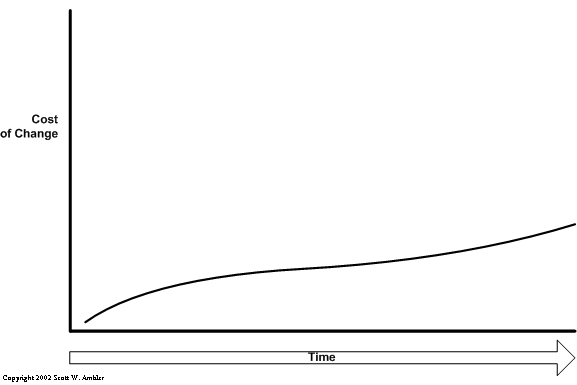
\includegraphics[width=0.6\textwidth]{figures/costOfChange}
\captionsetup{justification=centering}
\caption{Scott Amblers agile cost of change curve
\label{fig:costOfChange}}
\end{figure}

With this in mind this project aims to enable developers with limited
experience in web development to write cleaner, more semantic code. It is
through educating developers that the primary goal of offering a better
experience to users of assistive tools can be achieved.


By building a tool that can be used during
the development process the feedback loop on issues will be much
shorter and as described in agile 'cost of change' the cost of remediation
much lower. The tool will be supported by an accessibility guide which can
be used either to teach or to reference when trying to understand.

John Clifford a Senior Software Engineer at Capgemini has written a short
paragraph about Capgemini's need for a project in this area:
\begin{center}
\label{quote:john}
\textit{
``Front end development is known by many, but mastered by few. Software
engineers tend to have a good grasp of the basics, producing screens to meet
business requirements, but the skills required to make accessible systems are
often ignored completely.}

\textit{
Capgemini works on a number of projects in the public sector where
non-functional requirements will typically include adhering to Web Content
Accessibility Guidelines (WCAG). Whilst the guidelines themselves are clear,
they offer no practical examples/explanations of their implementation. For
developers unfamiliar with the subject the perceived difficulty of meeting the
guidelines and the small target audience is enough for them to want to delay
their implementation as much as possible. This feeds back into project
management, often resulting in the team opting to “add in accessibility later”.
Modifying a project that has not taken the WCAG into consideration throughout
its development can require large amounts of refactoring/rewriting, cause
unforeseen costs, and result in a solution that is of no real benefit to a user
using assistive software.}

\textit{
As a front end advocate, I feel that a guide and tool that can clearly
demonstrate and describe what implementing Web Accessibility looks like and its
importance to those that use rely on it would be a great benefit to Capgemini’s
developers and the developer community as a whole. If these guidelines could
be distilled into the kind of language that has become commonplace for
explaining other areas of front end development, it would help to dispel
myths of complexity and allow projects to implement WCAG in a meaningful way.
This would save on project costs by removing pitfalls of “adding it later”; but
importantly, it would help to keep the web a diverse and inclusive place."}
\end{center}

\section{Project Goals}
The core aim of this project is to make an impact in both Capgemini and the
wider web development community. By discovering the software
engineering communities needs first
the project deliverables will be relevant, useful and fill the described
business need. The deliverables are:
\begin{enumerate}
  \item A tool for software engineers which will bootstrap itself into a web
browser, assess and report possible accessibility issues
  \item A suite of documentation which will collate and demonstrate best
practices. It will show what 'assistive tools' output based upon different
HTML semantics. The current most popular tooling will be used to produce this.
  \item This report which will describe the journey, from researching the
topic, to designing and building the tool.
\end{enumerate}

\section{Project Stakeholders}
This project has a small number of stakeholders but a wide range of beneficiaries.
\begin{itemize}
  \item My two supervisors — Academic and Company, these are the people whom
  the deliverables will be presented too.
  \item Software Engineers at Capgemini — To improve the experience for the
  users web developers \& designers are those who need to produce a better
  product.
  \item Software Engineers within the wider community - Similar to above
  \item Users of assistive technologies. This whole project would be
    impossible and have no impact without them.
\end{itemize}

\section{Methodology}
Capgemini employees are encouraged to follow seven core values. Two of them
which stand out to me are ``Boldness" and ``Fun" \citep{CapValues}, it is these
two that drive me to try out new things in the aim of team (and consequently
self) improvement.

Although individual, this project serves as no exception and offers an
opportunity to experiment for the full duration of a project rather than a
few 'sprints' \citep{ScrumSprint}. These 'experiments' will be evaluated at the
end of the project for both myself and others to gain value from. Highlighted
below are a few aspects in which the traditional academic model for a
project will be broken and experimentation will prevail:
 \begin{itemize}
  \item Project Diary - Typically this is done on paper, or captured later in
   the project. 'Medium' \citep{Medium} a blogging platform will instead be
   used to
   capture key events and entries. At the end of the project this will be
   supplemented with notes from meetings between myself and my acadamic
   supervisor.
   %TODO - Check with HARRY if the below statement is correct. This is
   %TODO   currently an assumption and may be totally incorrect.
  \item Project Deliverables - The products of an academic project are usually
  completed in isolation or as part of a group and made available only upon
  completion of the project. Experimenting with ``Continuous Delivery"
  \citep{ContinuousDelivery}, products of this project will be delivered
  whilst still undergoing active development. This will enable 'faster
  feedback' from stakeholders and produce a higher quality product
  \item Open Source Everything - Capgemini consumes and
  produces a lot of open source software! With myself sitting within a team
  that are leading this drive, all code produced will be available under a MIT
  Licence \citep{MITLicence} on Github.
  \item Share Everything - The JVM team has its own 'ethos'
  \citep{JVMHowWeWork} that sits on top
  of Capgemini's core values one of these is to share knowledge within the
  company and the wider development community. This project will follow that
  ethos and everything will be available online.
  \item Automation - Another of the JVM teams 'values'. Repetitive boring tasks
  should be automated at the earliest possible chance! ``Deployment should be a
   repetitive boring task" \citep{ZachHolman} so this will be one of the first
   things
   tackled on
   each deliverable. This will allow its process to be tested and validated
   for every change made thereafter; reducing risk of failure later in the
   project. Travis CI \citep{TravisCi} and Github Pages \citep{Ghpages} will
   enable
   this.
 \end{itemize}

\subsection{Making Better Decisions}
% TODO * reference Agile Manifesto
Coming from a background in Agile projects, the ``Agile Manifesto" \citep{AgileManifesto} has
enabled
me to make and justify difficult decisions under pressure. For example deciding
 if a time constrained delivery should be moved into or out of the next
 sprint. One of the 'experiments' I wish to undertake is whether having such a
 manifesto makes a difference to a projects direction. With this in mind,
 within the evaluation I will discuss moments this was used and how I felt
 it affected the project. The manifesto for this project will be:

\begin{center}
Making an impact over getting a good grade

Hypothesis’ and supporting evidence over guessing and assuming

``Start simple with many organic iterations" over ``Upfront design"

Final Project over going to the pub
\end{center}

\subsection{A Process}
Capgemini projects always follow a process \citep{CapgeminiSustain} to ensure a
quality
product is delivered with the speed being measurable and quantifiable to
stakeholders and clients.

This project is no exception and will follow the Unified Process. This gives
a structure to different phases throughout the lifecycle of
the project Inception, Elaboration, Construction and Transition. It enables
iterations to occur within each of these phases but focuses the iteration
towards the goal of the phase you are currently in.

\subsubsection{Why the Unified Process?}

Agile is a poor fit for me as a distant learner with a
full time job. Each iteration requires a small amount of every aspect of the
development lifecycle (analysis, design, implementation and test). This would
make it difficult to understand and report progress to myself and the
stakeholders. Given the projects deliverables are well known from
the outset Agile would only add unneccesary ceremonies.

Using the manifesto above, the sprial model would satisfy ``Start simple with
many organic iterations", due to each turn of the spiral gaining user feedback
and then using that feedback to direct new requirements. It's flexible enough
 and well structured for this project. What steered the project towards Unified
 Process over Spiral was the amount of risk
collection and analysis required. Due to being an individual project, most
risks fall into the low probability, low impact category, and with one quater of
each spiral dedicated to risk analysis .

\subsection{High Level Planning}
At a high level I was aiming for the following to be acheived:
\begin{enumerate}
  \item {Inception - February}
    \begin{itemize}
      \item Identify ways of working
      \item Identify stakeholders
      \item Go out to charities and users and find the most common issues they face
      \item Identify the most common web ‘components’ (e.g. dialog)
      \item Understand how accessibility issues can be identified (in the IDE,
       in the browser?)
      \item Gather tools for testing hypothesis’
    \end{itemize}
  \item {Elaboration - March/Start of April}
    \begin {itemize}
      \item Use tools to assess common web ‘components’ on a range of sites
      \item Build these components as small web pages using common web frameworks.
      \item Produce more accessible friendly versions of all components
      \item Record and document the difference between how tools behave
      against these components
      \item Document how to’s and lessons learned
      \item Build A11Y Guide
    \end {itemize}
  \item {Construction - April/May}
    \begin{itemize}
      \item Design system for identifying issues in code
      \item Build \& Test a framework to enable identification of accessibility
      issues
      \item Build a small set of rules to demonstrate
    \end{itemize}
  \item {Transition - May}
     \begin{itemize}
        \item Document tool
        \item Gather feedback
     \end{itemize}
\end {enumerate}

\section{A Major Issue}
Due to unforseen circumstances \textasciitilde6 weeks of time was lost;
Mid-March through to the start of May. This covered the Elaboration, and
Construction phase of the project. So it was clear a change in process would be
necessary.

\subsection{Change of process}
I chose to change from the 'Unified Process' towards a more
prototypical/iterative process; 'Evolutionary Prototyping'. This is a form of
the prototyping model which often suits tight time scales and fast development
lifecycles \citep{EvoProto}. The 'Evoloutionary' aspect means rather than the
prototype being thrown away and rebuilt at the end, it will instead be
iteratively enhanced until a final product is produced. Fig.~\ref{fig:proto}
from \citep{EvoProto2} displays the process.

\begin{figure}[H]
\centering
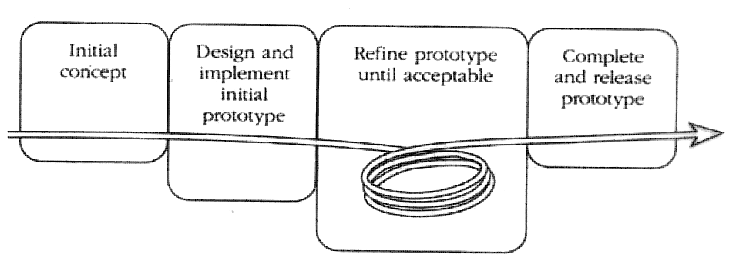
\includegraphics[width=0.6\textwidth]{figures/prototyping}
\captionsetup{justification=centering}
\caption{Evolutionary Prototyping
\label{fig:proto}}
\end{figure}

Using this method will enable the code and project to carry some technical debt
whilst still using continuous delivery. There is a higher
risk to the quality of the product but as this is an individual process I am in
control of that and thus it will be consistent. All technical debt
accumulated and areas for improvement will be documented in the
deliverable/evaluation section respectively.
